%!TEX root = ../main.tex
\section{Augmenting path algorithms}
\subsection{Introduction}
The idea behind the augmenting path algorithms is as follows : 
As long as there is a path from the source to the sink, we send flow along this path. And so on until there is no more path from the source to the sink. \newline

A directed path from the source to the sink in the \textit{residual network} is called \textit{augmenting path}. For instance here is a network with its \textit{residual network}: \newline

\begin{figure}[!h]
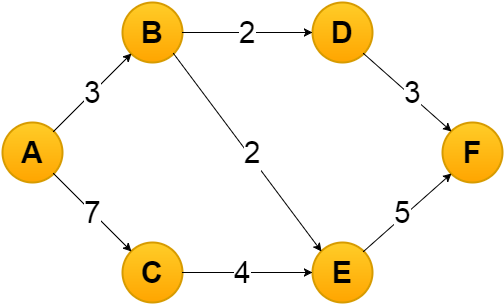
\includegraphics[width=7.5cm,height=4.5cm]{images/graph.png}\hfill
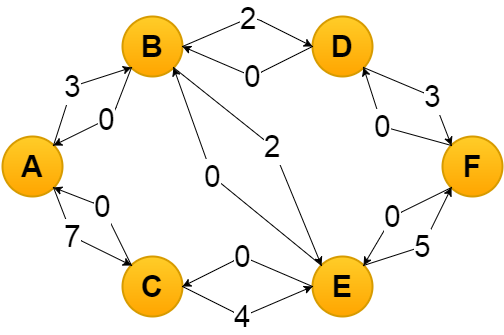
\includegraphics[width=7.5cm,height=4.5cm]{images/residualgraph.png}
\caption{A network with its residual graph.}
\end{figure}


When an \textit{augmenting path} is found, we send a flow equivalent to the minimum capacity of any edge in the path. We update the \textit{residual network} by decreasing capacities in forward edges and increasing capacities in backward edges. Then we look for a new augmenting path in the new \textit{residual network}. \newline

Here is the \textit{residual network} after sending 4 units of flow through the \textit{augmenting path} A-C-E-F : \newline

\begin{center}
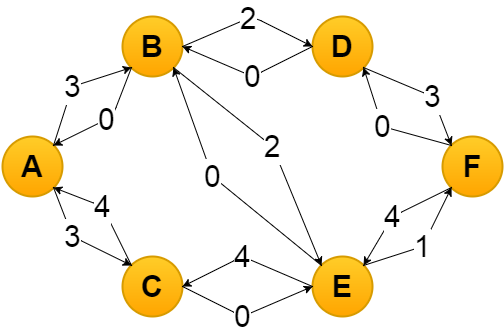
\includegraphics[width=7.5cm,height=4.5cm]{images/residualgraph2.png}
\captionof{figure}{Residual graph}
\end{center}

The pseudo-code of the augmenting path algorithm is given here :

\begin{algorithm}[h]

 \While{$G_f$ contains a directed path from node s to node t}{
  identify an augmenting path P from node s to node t\;
  $\delta$ = min\{$c_{ij} : (i,j) \in P$\}\;
  augment $\delta$ units of flow along P and update $G_f$\;
 }
\end{algorithm}

\subsection{Ford-Fulkerson and Edmonds-Karp}
There are two main augmenting path algorithms, Ford-Fulkerson (published in 1956) and Edmonds-Karp (published in 1972). The second being a variant of the first one. Indeed, the unique difference between both is the way of looking for an \textit{augmenting path} in the \textit{residual network}. \newline

Ford-Fulkerson uses a depth-first search, looking for the longest path. The flow is thus sent on a large number of edges but a small quantity. Indeed, a long path have a higher chance to contains at least one edge with a low capacity. \newline

While Edmonds-Karp uses a breadth-first search, looking for the shortest path. A bigger quantity of flow is thus sent on a smaller number of edges. \newline


\subsection{Complexities}
The max flow problem, being a problem of complexity class P, can be solved at polynomial time. When the capacities are integers, Ford-Fulkerson is bounded by $O(|E|*|f|)$ and Edmonds-Karp by $O(|V|*|E|^2)$, where $|E|$ is the number of edges in the graph, $|V|$ is the number of vertices and $|f|$ is the value of the flow.

\begin{description}
\item[Ford-Fulkerson]{is in $O(|E|*|f|)$ because each augmenting path can be found in $O(|E|)$ thanks to the depth-first search algorithm and in the worst case, the flow will increase by 1.}
\item[Edmonds-Karp]{is in $O(|V|*|E|^2)$ because the breadth-first search assures us that after each iteration, the length of the augmenting path can't decrease. Futhermore, the length of the augmenting path can stay the same for at most $|E|$ iterations before increasing. We also know that the length of the augmenting path is between $1$ and $|V|-1$. Thus there are at most $|V|*|E|$ iterations and each augmenting path can be found in $O(|E|)$.}
\end{description}


\section{Preflow-push algorithms}

\subsection{Introduction}

The drawback of the augmenting path algorithms is the operation of sending flow along a path. The time complexity of this operation in the worst case is $O(n)$, where $n$ is the number of vertcices in the augmenting path. One example of this case can be seen in the figure \ref{img:bad_augmenting}. With augmenting path algorithms, only one unit of flow can be pushed at a time on the network represented in the figure \ref{img:bad_augmenting}. In this case, a better solution is to push directly from the source node 10 units of flow. This is the idea behing preflow-push algorithms.

\begin{figure}
\centering
\includegraphics[scale=0.5]{images/bad_augmenting.png}
\caption{Extreme case for augmenting path algorithms.}
\label{img:bad_augmenting}
\end{figure}

The preflow-push algorithms don't push flow on augmenting path, they push flow on individual vertices. Because of this, preflow-push algorithms does not respect the flow conservation constraint. Indeed, these algorithms permit the flow entering a node to exceed the flow leaving the node. We call this flow a preflow.

\begin{definition}
\label{preflow}
A \textbf{preflow} is a function $x: E \to \mathbb{R}$ that satisfies the capacity constraint and the following relaxation of the flow conservation constraint:
$$\sum\limits_{\{j : (j,i) \in E\}} x_{ji} - \sum\limits_{\{j : (i,j) \in E\}} x_{ij} \geq 0 \text{	for each } i \in V \setminus \{s, t\}.$$
\end{definition}

\begin{definition}
\label{excess}
The \textbf{excess} of each node $i \in V$ is 
$$e(i) = \sum\limits_{\{j : (j,i) \in E\}} x_{ji} - \sum\limits_{\{j : (i,j) \in E\}} x_{ij}.$$
\end{definition}

We call a node with positive excess as an \textbf{active node}. The fact that there are active nodes means that the current solution is not feasible. Thus, the goal of the algorithm is to remove the excess from those nodes. The intuition is to push the flow to the node closer to the sink. Each node has its own distance label which is the distance between the node and the sink: the algorithm only push a flow from a node to another if the first one is an active node and if his distance label if greater than the distance label of the other node. This operation is called a \textbf{push operation}. If such scenario cannot be applied, we need to relabel the distance label of the node. This operation is called the \textbf{relabel operation}. The algorithm terminates when there is no more active node.

\begin{algorithm}
 preprocess\;
 \While{the network contains an active node}{
 select an active node $i$\;
 push/relabel($i$)\;
 }
\caption{Generic preflow-push algorithm.}
\end{algorithm}

\begin{algorithm}
 $x\gets 0$\;
 compute distance labels $d(i)$\;
 $x_{sj}\gets c_{sj} \text{ for each arc } (s, j) \in E(s)$\;
 $d(s)\gets v$\;
\caption{Preprocess.}
\end{algorithm}

\begin{algorithm}
\If{the network contains an admissible arc $(i, j)$} 
  {push $\delta\gets min\{e(i), r_{ij}\}$ units of flow from $i$ to $j$\;}
\Else
   {replace $d(i)$ by $min\{d(j)+1 : (i, j) \in E(i) \text{ and } r_{ij} > 0 \}$\;}
\caption{Push/Relabel($i$).}
\end{algorithm}

\subsection{Complexity}

There is a possibility of maximum $|V|^2$ relabel operations. This is because the maximum distance is $2*|V| - 1$ and we can decrease the label distance at minimum one per operation. We know that there is $|V| - 2$ nodes which can be relabeled (the sink and source nodes can't be relabeled). Then, the maximum number of relabelling is $(2*|V| - 1) * (|V| - 2) \approx |V|^2$.%todo why distance 2V-1

The number of saturing push per edge is $O(|V|)$. To make a saturing push on a certain edge again, the label distance of the destination node must be augmented of 2. Then there is $O(\frac{2*|V| - 1}{2}) \approx O(|V|)$ saturing push per edge: the number of maximum saturing push is $O(|V||E|)$.

Thus, the generic preflow algorithm runs in $O(|V|^2 |E|)$. %todo